% Options for packages loaded elsewhere
\PassOptionsToPackage{unicode}{hyperref}
\PassOptionsToPackage{hyphens}{url}
\PassOptionsToPackage{dvipsnames,svgnames,x11names}{xcolor}
%
\documentclass[
  letterpaper,
  DIV=11,
  numbers=noendperiod]{scrartcl}

\usepackage{amsmath,amssymb}
\usepackage{iftex}
\ifPDFTeX
  \usepackage[T1]{fontenc}
  \usepackage[utf8]{inputenc}
  \usepackage{textcomp} % provide euro and other symbols
\else % if luatex or xetex
  \usepackage{unicode-math}
  \defaultfontfeatures{Scale=MatchLowercase}
  \defaultfontfeatures[\rmfamily]{Ligatures=TeX,Scale=1}
\fi
\usepackage{lmodern}
\ifPDFTeX\else  
    % xetex/luatex font selection
\fi
% Use upquote if available, for straight quotes in verbatim environments
\IfFileExists{upquote.sty}{\usepackage{upquote}}{}
\IfFileExists{microtype.sty}{% use microtype if available
  \usepackage[]{microtype}
  \UseMicrotypeSet[protrusion]{basicmath} % disable protrusion for tt fonts
}{}
\makeatletter
\@ifundefined{KOMAClassName}{% if non-KOMA class
  \IfFileExists{parskip.sty}{%
    \usepackage{parskip}
  }{% else
    \setlength{\parindent}{0pt}
    \setlength{\parskip}{6pt plus 2pt minus 1pt}}
}{% if KOMA class
  \KOMAoptions{parskip=half}}
\makeatother
\usepackage{xcolor}
\setlength{\emergencystretch}{3em} % prevent overfull lines
\setcounter{secnumdepth}{-\maxdimen} % remove section numbering
% Make \paragraph and \subparagraph free-standing
\makeatletter
\ifx\paragraph\undefined\else
  \let\oldparagraph\paragraph
  \renewcommand{\paragraph}{
    \@ifstar
      \xxxParagraphStar
      \xxxParagraphNoStar
  }
  \newcommand{\xxxParagraphStar}[1]{\oldparagraph*{#1}\mbox{}}
  \newcommand{\xxxParagraphNoStar}[1]{\oldparagraph{#1}\mbox{}}
\fi
\ifx\subparagraph\undefined\else
  \let\oldsubparagraph\subparagraph
  \renewcommand{\subparagraph}{
    \@ifstar
      \xxxSubParagraphStar
      \xxxSubParagraphNoStar
  }
  \newcommand{\xxxSubParagraphStar}[1]{\oldsubparagraph*{#1}\mbox{}}
  \newcommand{\xxxSubParagraphNoStar}[1]{\oldsubparagraph{#1}\mbox{}}
\fi
\makeatother

\usepackage{color}
\usepackage{fancyvrb}
\newcommand{\VerbBar}{|}
\newcommand{\VERB}{\Verb[commandchars=\\\{\}]}
\DefineVerbatimEnvironment{Highlighting}{Verbatim}{commandchars=\\\{\}}
% Add ',fontsize=\small' for more characters per line
\usepackage{framed}
\definecolor{shadecolor}{RGB}{241,243,245}
\newenvironment{Shaded}{\begin{snugshade}}{\end{snugshade}}
\newcommand{\AlertTok}[1]{\textcolor[rgb]{0.68,0.00,0.00}{#1}}
\newcommand{\AnnotationTok}[1]{\textcolor[rgb]{0.37,0.37,0.37}{#1}}
\newcommand{\AttributeTok}[1]{\textcolor[rgb]{0.40,0.45,0.13}{#1}}
\newcommand{\BaseNTok}[1]{\textcolor[rgb]{0.68,0.00,0.00}{#1}}
\newcommand{\BuiltInTok}[1]{\textcolor[rgb]{0.00,0.23,0.31}{#1}}
\newcommand{\CharTok}[1]{\textcolor[rgb]{0.13,0.47,0.30}{#1}}
\newcommand{\CommentTok}[1]{\textcolor[rgb]{0.37,0.37,0.37}{#1}}
\newcommand{\CommentVarTok}[1]{\textcolor[rgb]{0.37,0.37,0.37}{\textit{#1}}}
\newcommand{\ConstantTok}[1]{\textcolor[rgb]{0.56,0.35,0.01}{#1}}
\newcommand{\ControlFlowTok}[1]{\textcolor[rgb]{0.00,0.23,0.31}{\textbf{#1}}}
\newcommand{\DataTypeTok}[1]{\textcolor[rgb]{0.68,0.00,0.00}{#1}}
\newcommand{\DecValTok}[1]{\textcolor[rgb]{0.68,0.00,0.00}{#1}}
\newcommand{\DocumentationTok}[1]{\textcolor[rgb]{0.37,0.37,0.37}{\textit{#1}}}
\newcommand{\ErrorTok}[1]{\textcolor[rgb]{0.68,0.00,0.00}{#1}}
\newcommand{\ExtensionTok}[1]{\textcolor[rgb]{0.00,0.23,0.31}{#1}}
\newcommand{\FloatTok}[1]{\textcolor[rgb]{0.68,0.00,0.00}{#1}}
\newcommand{\FunctionTok}[1]{\textcolor[rgb]{0.28,0.35,0.67}{#1}}
\newcommand{\ImportTok}[1]{\textcolor[rgb]{0.00,0.46,0.62}{#1}}
\newcommand{\InformationTok}[1]{\textcolor[rgb]{0.37,0.37,0.37}{#1}}
\newcommand{\KeywordTok}[1]{\textcolor[rgb]{0.00,0.23,0.31}{\textbf{#1}}}
\newcommand{\NormalTok}[1]{\textcolor[rgb]{0.00,0.23,0.31}{#1}}
\newcommand{\OperatorTok}[1]{\textcolor[rgb]{0.37,0.37,0.37}{#1}}
\newcommand{\OtherTok}[1]{\textcolor[rgb]{0.00,0.23,0.31}{#1}}
\newcommand{\PreprocessorTok}[1]{\textcolor[rgb]{0.68,0.00,0.00}{#1}}
\newcommand{\RegionMarkerTok}[1]{\textcolor[rgb]{0.00,0.23,0.31}{#1}}
\newcommand{\SpecialCharTok}[1]{\textcolor[rgb]{0.37,0.37,0.37}{#1}}
\newcommand{\SpecialStringTok}[1]{\textcolor[rgb]{0.13,0.47,0.30}{#1}}
\newcommand{\StringTok}[1]{\textcolor[rgb]{0.13,0.47,0.30}{#1}}
\newcommand{\VariableTok}[1]{\textcolor[rgb]{0.07,0.07,0.07}{#1}}
\newcommand{\VerbatimStringTok}[1]{\textcolor[rgb]{0.13,0.47,0.30}{#1}}
\newcommand{\WarningTok}[1]{\textcolor[rgb]{0.37,0.37,0.37}{\textit{#1}}}

\providecommand{\tightlist}{%
  \setlength{\itemsep}{0pt}\setlength{\parskip}{0pt}}\usepackage{longtable,booktabs,array}
\usepackage{calc} % for calculating minipage widths
% Correct order of tables after \paragraph or \subparagraph
\usepackage{etoolbox}
\makeatletter
\patchcmd\longtable{\par}{\if@noskipsec\mbox{}\fi\par}{}{}
\makeatother
% Allow footnotes in longtable head/foot
\IfFileExists{footnotehyper.sty}{\usepackage{footnotehyper}}{\usepackage{footnote}}
\makesavenoteenv{longtable}
\usepackage{graphicx}
\makeatletter
\def\maxwidth{\ifdim\Gin@nat@width>\linewidth\linewidth\else\Gin@nat@width\fi}
\def\maxheight{\ifdim\Gin@nat@height>\textheight\textheight\else\Gin@nat@height\fi}
\makeatother
% Scale images if necessary, so that they will not overflow the page
% margins by default, and it is still possible to overwrite the defaults
% using explicit options in \includegraphics[width, height, ...]{}
\setkeys{Gin}{width=\maxwidth,height=\maxheight,keepaspectratio}
% Set default figure placement to htbp
\makeatletter
\def\fps@figure{htbp}
\makeatother

\KOMAoption{captions}{tableheading}
\makeatletter
\@ifpackageloaded{caption}{}{\usepackage{caption}}
\AtBeginDocument{%
\ifdefined\contentsname
  \renewcommand*\contentsname{Table of contents}
\else
  \newcommand\contentsname{Table of contents}
\fi
\ifdefined\listfigurename
  \renewcommand*\listfigurename{List of Figures}
\else
  \newcommand\listfigurename{List of Figures}
\fi
\ifdefined\listtablename
  \renewcommand*\listtablename{List of Tables}
\else
  \newcommand\listtablename{List of Tables}
\fi
\ifdefined\figurename
  \renewcommand*\figurename{Figure}
\else
  \newcommand\figurename{Figure}
\fi
\ifdefined\tablename
  \renewcommand*\tablename{Table}
\else
  \newcommand\tablename{Table}
\fi
}
\@ifpackageloaded{float}{}{\usepackage{float}}
\floatstyle{ruled}
\@ifundefined{c@chapter}{\newfloat{codelisting}{h}{lop}}{\newfloat{codelisting}{h}{lop}[chapter]}
\floatname{codelisting}{Listing}
\newcommand*\listoflistings{\listof{codelisting}{List of Listings}}
\makeatother
\makeatletter
\makeatother
\makeatletter
\@ifpackageloaded{caption}{}{\usepackage{caption}}
\@ifpackageloaded{subcaption}{}{\usepackage{subcaption}}
\makeatother

\ifLuaTeX
  \usepackage{selnolig}  % disable illegal ligatures
\fi
\usepackage{bookmark}

\IfFileExists{xurl.sty}{\usepackage{xurl}}{} % add URL line breaks if available
\urlstyle{same} % disable monospaced font for URLs
\hypersetup{
  pdftitle={Sustainability},
  colorlinks=true,
  linkcolor={blue},
  filecolor={Maroon},
  citecolor={Blue},
  urlcolor={Blue},
  pdfcreator={LaTeX via pandoc}}


\title{Sustainability}
\author{}
\date{}

\begin{document}
\maketitle


\subsection{Evolving Sustainability Measurments from Planetary
Boundaries to Planetary
Health}\label{evolving-sustainability-measurments-from-planetary-boundaries-to-planetary-health}

\emph{Sustainability} was first mentioned in the seminal book
\emph{Sylvicultura oeconomica} in the context of forestry with the goal
of achieving sustainable forest management (Hannß Carl von Carlowitz,
1713). The field is known today as \emph{sustainable yield} of
\emph{natural capital} with a focus on maintaining \emph{ecosystem
services} (Peter Kareiva et al., 2011). Aldo Leopold proposed the idea
of \emph{land ethics} as \emph{``{[}a{]} thing is right when it tends to
preserve the integrity, stability, and beauty of the biotic community.
It is wrong when it tends otherwise''} in his landmark work \emph{A Sand
County Almanac} (Leopold, 1972). The 1987 United Nations' Brundtland
Report (Our Common Future) defined sustainable development as
\emph{``Development that meets the needs of the present without
compromising the ability of future generations to meet their own
needs''} (World Commission on Environment and Development, 1987).

In 1896, the Nobel Prize winner Svante Arrhenius first calculated how an
increase in CO\textsubscript{2} levels could have a warming effect on
our global climate (Anderson, Hawkins and Jones, 2016; Wulff, 2020). 120
years later, the Paris Climate Agreement came into effect, with
countries agreeing on non-binding targets on how to keep
CO\textsubscript{2} levels 1.5 °C below pre-industrial levels (United
Nations, 2016). While awareness of Earth's warming climate was growing,
the CO\textsubscript{2} emissions kept rising too. The hockey-stick
growth of CO\textsubscript{2} concentration since the industrial
revolution is clear in the data from 1958 onward, following a steady
annual increase, called the \emph{Keeling Curve} (Keeling and Keeling,
2017). Written records of global temperature measurements are available
starting from the 1880s when documentation of temperatures become
available in ship records (Brohan et al., 2012). Temperature estimations
from tree-trunks allow some temperature comparisons with the climate as
far back as 2000 years ago (Rubino et al., 2019).

\begin{figure}[H]

{\centering \includegraphics{./images/co2-concentration.png}

}

\caption{CO\textsubscript{2} concentration in the atmosphere as of Ap.
Image Credit: Scripps Institution of Oceanography at UC San Diego.}

\end{figure}%

In 1938, Guy Stewart Callendar was the first to demonstrate the warming
of Earth's land surface as well as linking the production of fossil
fuels to increased CO\textsubscript{2} and changing climate (Hawkins and
Jones, 2013). By the latest data from 2022, the current world population
of 8 Billion people emitted 37.5 gigatonnes of CO\textsubscript{2} per
year, the highest emissions recorded in history (Statista, 2023). To
limit global warming to 1.5 °C as agreed by the world nations in Paris,
removal of 5-20 gigatons of CO\textsubscript{2} per year would be needed
according to reduction pathways calculated by the Intergovernmental
Panel on Climate Change (IPCC) (Wade et al., 2023). Yet, most countries
are missing the mark. Given this model of climate change, the G7
countries (Canada, France, Germany, Italy, Japan, United Kingdom, United
States) are heading for 2.7 °C of warming by 2050 (CDP, 2022). The
monumental task of removing several gigatons of CO\textsubscript{2} from
the atmosphere requires massive policy shifts and collaboration across
countries and industries (Mackler, Fishman and Broberg, 2021).

News reports saying quoting the ``The European Union's Copernicus
Climate Change Service (C3S)'' 1.5 has already been breached (Anon.,
2024a; Anon., 2024b).

In 1948, the International Union for Conservation of Nature (IUCN) was
founded, which in

LULUCF ``Land Use, Land-Use Change, and Forestry'' can be a source of
greenhouse gas emissions or a carbon sink (removing CO2 from the
atmosphere)

\begin{figure}[H]

{\centering \includegraphics[width=0.8\textwidth,height=\textheight]{./images/boundaries.png}

}

\caption{Planetary Boundaries. J. Lokrantz/Azote based on Steffen et
al.~2015}

\end{figure}%

In addition the enormity of emissions, humanity is facing other massive
problems. The Stockholm Resilience Centre reports we have already
breached 4 out of our 9 planetary boundaries: in addition to climate
change, biodiversity loss (Extinctions per Million Species per Year aka
E/MSY), land-system change (deforestation, land degradation, etc), and
biogeochemical flows (cycles of carbon, nitrogen, phosphorus, etc); on a
positive side, the challenges of fresh water use, ocean acidification
and stratospheric ozone depletion are still within planetary limits
(Persson et al., 2022).

Atmospheric aerosol loading and the biodiversity intactness index (BII)
were quantified recently (ADD CITATION)

\begin{itemize}
\tightlist
\item
  (Keeble, 1988) reported in April 1987 that \emph{`residents in
  high-income countries lead lifestyles incompatible with planetary
  boundaries'}. While my home country Estonia at the time was considered
  low-income, a small nation in poverty behind the \emph{Iron Curtain}
  occupation of the Soviet Occupy, we now in 2023, have indeed reached
  high-income status.
\item
  De Balie (2018)
\item
  Houdini (2018)
\item
  Haeggman, Moberg and Sandin (2018)
\end{itemize}

\paragraph{Planetary Boundaries}\label{planetary-boundaries}

\begin{itemize}
\tightlist
\item
  As long as humanity is a mono-planetary species, we have to come to
  terms with the limitations of our home, Earth.
\end{itemize}

\subsubsection{Planetary Health}\label{planetary-health}

\begin{itemize}
\item
  Planetary health
  https://unfccc.int/climate-action/un-global-climate-action-awards/planetary-health
\item
  Wardani et al. (2023) \emph{``long-term human well-being is dependent
  on the well-being of the planet, including both biotic and abiotic
  systems. It recognizes interlinkages across environmental
  sustainability, public health, and socioeconomic development.''}
\end{itemize}

\subsubsection{Biodiversty Loss}\label{biodiversty-loss}

Protecting biodiversity

\begin{longtable}[]{@{}
  >{\raggedright\arraybackslash}p{(\columnwidth - 2\tabcolsep) * \real{0.6234}}
  >{\raggedright\arraybackslash}p{(\columnwidth - 2\tabcolsep) * \real{0.3766}}@{}}
\caption{Biodiversity loss data from (Bradshaw et al.,
2021).}\tabularnewline
\toprule\noalign{}
\endfirsthead
\endhead
\bottomrule\noalign{}
\endlastfoot
What Happened? & How Much? \\
Vertebrate species population average decline & 68\% over the last 50
years \\
Land surface altered by humans & 70\% of Earth \\
Vertebrate species extinct & 700 in 500 years \\
Plant species extinct & 600 in 500 years \\
Species under threat of extinction & 1 million \\
\end{longtable}

\begin{itemize}
\tightlist
\item
  The current environmental upheaval, led by Gen-Z and Millennials, and
  the business adaptation (or lack thereof) to sustainable economic
  models, taking into account the hidden social and environmental costs
  we didn't calculate in our pricing before.
\item
  We also need to consider environmental effects (E in ESG). We haven't
  taken into account the whole cost of production, leading to the wrong
  pricing information. To achieve this, we need expert governance (G).
\end{itemize}

Consumer lifestyle contributes to environmental destruction. According
to Ellen MacArthur Foundation, Material Economics (2019)'s models show
45\% of CO\textsubscript{2} equivalent emissions come from our shopping;
produced by companies to make the products we consume. A large scale
study by Anthony Leiserowitz et al. (2022) on Meta's Facebook (n=108946)
reported people in Spain (65\%), Sweden (61\%), and Taiwan (60\%)
believe \emph{``climate change is mostly caused by human activities''.}
An even larger survey (n=1.2 million) by the United Nations across 50
countries, distributed through mobile game ads, showed the majority of
people agreeing climate change is an ``emergency'' UNDP (2021). While
people express eco-conscious ideas, it's non-trivial to practice
sustainability in daily life. Deyan Georgiev (2023) reports only 30\% of
people in the Gen-Z age group believe technology can solve all problems.

\begin{longtable}[]{@{}lll@{}}
\caption{``Climate change is an emergency'' UNDP (2021).}\tabularnewline
\toprule\noalign{}
\endfirsthead
\endhead
\bottomrule\noalign{}
\endlastfoot
Age Group & Agree & Neutral or Disagree \\
18-35 & 65\% & 35\% \\
36-59 & 66\% & 34\% \\
Over 69 & 58\% & 42\% \\
\end{longtable}

AI is being used to maps icebergs and measure the change in size
European Space Agency (2023)

\subsection{Ecological Indicators of the
Biosphere}\label{ecological-indicators-of-the-biosphere}

Sustainability can be measured using a variety of
\textbf{\emph{ecological indicators}}.

Dinerstein et al. (2017) identifies 846 terrestrial ecoregions.

\begin{itemize}
\tightlist
\item
  Svalbard Seed Vault
\item
  Jackson (1996) \emph{preventive environmental management}
\item
  Jackson (2017) limits to growth update
\item
  Ecological Indicators (I like the name Ecomarkers) for Earth are like
  Biomarkers in human health.
\end{itemize}

Some argue sustainability is not enough and we should work on
regeneration of natural habitats.

\subsubsection{The Climate}\label{the-climate}

\paragraph{The Price of Climate
Change}\label{the-price-of-climate-change}

Long term cost is more than short-term gains.

\paragraph{Climate Data Vizualisation}\label{climate-data-vizualisation}

Climate data visualization has a long history, starting with
\textbf{\emph{Alexander von Humboldt,}} the founder of climatology, who
revolutionized cartography by inventing the first \emph{isothermal maps}
around the year 1816; these maps showed areas with similar temperature,
variations in altitude and seasons in different colors (Honton, 2022).
Humboldt's isotherms are now available as 3D computer models in (Anon.,
2023a).

Earth's physical systems are very sensitive to small changes in
temperature, which was not understood until 30 years ago (McKibben,
2006).

\begin{itemize}
\tightlist
\item
  Industrial revolution: : ``transition to a low carbon economy presents
  challenges and potential economic benefits that are comparable to
  those of previous industrial revolutions'' (Pearson and Foxon, 2012).
\item
  Tragedy of the commons: (Murase and Baek, 2018; Lopez, Pastén and
  Gutiérrez Cubillos, 2022; Meisinger, 2022).
\end{itemize}

\begin{figure}[H]

{\centering \includegraphics[width=0.6\textwidth,height=\textheight]{./images/humboldt.jpg}

}

\caption{Humboldt's Naturgemälde, early data visualization of ecology,
rain, temperature, elevation, etc}

\end{figure}%

Earth System Models from the first calculation by Svante Arrhenius and
Guy Stewart Callendar to today's complex models that integrate the
various Earth systems and cycles ran on supercomputers Anderson, Hawkins
and Jones (2016)

\subsubsection{Climatech}\label{climatech}

How are large corporations responding to the climate crisis?

Lack of leadership. Capgemini (2022): ``Many business leaders see
sustainability as costly obligation rather than investment in the
future''. Hoikkala (2019): for example the CEO of the Swedish clothing
producer H\&M, one of the largest fast-fashion in the world, recognizes
the potential impact of conscious consumers as a threat.

Many large businesses have tried to find solutions by launching
climate-focused funding. (Korosec, 2021) reports that Amazon's 2B USD to
a Climate Pledge Fund earmarked to fix climate problems is invested in
energy, logistics, and packaging startups, which will reduce material
waste. ``Good intentions don't work, mechanisms do,'' Amazon's founder
Bezos is quoted as saying in (Clifford, 2022). Walmart is taking a
similar approach, having launched a project in 2017 to set
CO\textsubscript{2} reduction targets in collaboration with its
suppliers Walmart (2023). These examples underlines how money marketed
as climate funding by retail conglomerates means focus on reducing
operational cost of running their business through automation and
material savings.

Large corporations such as Nestle and Coca Cola support the biodiversity
law to have a level playing field for business (Greens EFA, 2023).

\begin{itemize}
\item
  Anon. (2013)
\item
  Guidotti (2015)
\item
  ``Sustainability is important for many reasons including:
  Environmental Quality --~In order to have healthy communities, we need
  clean air, natural resources, and a nontoxic environment.''
\item
  Low, S., Baum and Sovacool (2022) finds considerable uncertainty
  exists among experts which CO2 reduction methods among nature-based
  and technology-based are the most effective.
\item
  Pathways to drawdown
\end{itemize}

\subsubsection{Ecosystem Services Enable Life on
Earth}\label{ecosystem-services-enable-life-on-earth}

Gómez-Baggethun et al. (2010) the history of the valuation of nature's
services goes back to the 18th century when David Ricardo and Jean
Baptiste Say discussed nature's \emph{work}, however both considered it
should be free. In 1997 Daily (1997) proposed the idea of ecosystem
services and Costanza et al. (1997) attempted to assess the amount of
ecosystem services provided.

Le Provost et al. (2022) study shows \emph{biodiversity} as one key
factor to maintain delivery of ecosystem services. Noriega et al. (2018)
attempts to quantify the ecosystem services (ES) provided by insects.
While it can be assumed much of the flora and fauna are crucial for
Earth's systems, science is still in the process of understanding and
quantifying its contributions.

\begin{itemize}
\tightlist
\item
  Leverhulme Centre for Nature Recovery (2023) should we put a price on
  nature?
\item
  Bousfield et al. (2022) reports there's evidence paying landowners for
  the ecosystem services their forests provide may reduce deforestation.
\item
  Is it time to leave utilitarian environmentalism behind? Muradian and
  Gómez-Baggethun (2021)
\end{itemize}

\begin{longtable}[]{@{}l@{}}
\caption{From Leverhulme Centre for Nature Recovery
(2023)}\tabularnewline
\toprule\noalign{}
\endfirsthead
\endhead
\bottomrule\noalign{}
\endlastfoot
9 Steps \\
Identify ecosystem functions \\
Quantify ecosystem functions \\
Identify ecosystem services \\
Quantify ecosystem services \\
Quantify financial value of ecosystem services \\
Assign property rights \\
Create ecosystem service markets \\
Commodify nature \\
\end{longtable}

There are 2 approaches to protecting nature

\begin{longtable}[]{@{}
  >{\raggedright\arraybackslash}p{(\columnwidth - 2\tabcolsep) * \real{0.2222}}
  >{\raggedright\arraybackslash}p{(\columnwidth - 2\tabcolsep) * \real{0.7778}}@{}}
\toprule\noalign{}
\endhead
\bottomrule\noalign{}
\endlastfoot
Economics of Nature Commodification & Economics of the Sacred \\
Measure and assign value to nature & Say nature is sacred, such as
Churches, and can't be touched (Eisenstein, 2011, 2018) \\
& \\
& \\
\end{longtable}

\begin{itemize}
\tightlist
\item
  Han and Chen (2022) identifies nature-based solutions ``land
  re-naturalization (such as afforestation and wetland restoration)''
\end{itemize}

\begin{longtable}[]{@{}l@{}}
\caption{From Han and Chen (2022)}\tabularnewline
\toprule\noalign{}
Non-Exhaustive list of \\
\midrule\noalign{}
\endfirsthead
\toprule\noalign{}
Non-Exhaustive list of \\
\midrule\noalign{}
\endhead
\bottomrule\noalign{}
\endlastfoot
Afforestation \\
Wetland restoration \\
 \\
\end{longtable}

\begin{itemize}
\item
  Meanwhile the destruction pressure on ecosystems is rapidly increasing
  (ADD CITATION A B C).
\item
  Espinosa and Bazairi (2023) marine ecosystem services \textbf{(need
  access, ncku doesn't sub)}
\item
  Chen et al. (2023) Ecosystem vulnerability \textbf{(need access)}
\item
  Zhang et al. (2023) Integrating ecosystem services conservation into
  urban planning \textbf{(need access)}
\item
  Li et al. (2023) tourism is a large industrial sector which relies on
  ecosystem services. In Taiwan, (Lee, Jan and Liu, 2021) developed a
  framework of indicators to assess sustainable tourism.
\end{itemize}

\subsubsection{\texorpdfstring{\textbf{Environmental Degradation Is
Cir}}{Environmental Degradation Is Cir}}\label{environmental-degradation-is-cir}

\paragraph{Growing Population and
Overpopulation}\label{growing-population-and-overpopulation}

Earth's population reached 8 Billion people In November 2022 and
population projections by predict 8.5B people by 2030 and 9.7B by 2050
(The Economic Times, 2022; United Nations Department of Economic and
Social Affairs, Population Division, 2022).

(Hassoun et al., 2023) forecasts increase of global food demand by 62\%
including impact of climate change.

\begin{itemize}
\item
  While population growth puts higher pressure on Earth's resources,
  some research proposes the effect is more from wasteful lifestyles
  than the raw number of people (Cardinale et al., 2012).
\item
  Bowler et al. (2020) Anthropogenic Threat Complexes (ATCs):
\item
  ``Overpopulation is a major cause of biodiversity loss and smaller
  human populations are necessary to preserve what is left'' Cafaro,
  Hansson and Götmark (2022).
\end{itemize}

\paragraph{Marine Heatwaves}\label{marine-heatwaves}

\begin{itemize}
\tightlist
\item
  Gelles and Andreoni (2023) describe how marine heatwaves threaten
  global biodiversity.
\end{itemize}

\paragraph{Slavery Still Exists}\label{slavery-still-exists}

In 2023, an estimated 50 million people are still in slavery around the
world; lack of supply chain visibility hides forced labor and
exploitation of undocumented migrants in agricultural work; 71\% of
enslaved people are estimated to be women. (Borrelli et al., 2023; Kunz
et al., 2023).

The UN SDG target 8.7 targets to eliminate all forms of slavery.

Slavery is connected to environmental degradation and climate change
(Decker Sparks et al., 2021). Enslaved people are used in environmental
crimes such as 40\% of deforestation globally. Cobalt used in
technological products is in risk of being produced under forced labor
in the D.R. Congo (Sovacool, 2021). In India and Pakistan, forced labor
in brick kiln farms is possible to capture remotely from satellite
images (Boyd et al., 2018). In effect, the need for cheap labor turns
slavery into a \emph{subsidy} keeping environmental degradation
happening.

\begin{itemize}
\item
  Christ and V Helliar (2021) estimates 20 million people are stuck
  inside corporate blockchains. The Global Slavery Index measures the
  \textbf{\emph{Import Risk}} of having slavery inside its imports Walk
  Free (2023).
\item
  Hans van Leeuwen (2023) slavery affects industries from fashion to
  technology, including sustainability enablers such as solar panels.
\item
  ``commodification of human beings''
\item
  Anand Chandrasekhar and Andreas Gefe (2021): Trading commodities
  ``Switzerland has a hand in over 50\% of the global trade in coffee
  and vegetable oils like palm oil as well as 35\% of the global volume
  of cocoa, according to government estimates.'' Can traders have more
  scrutiny over what they trade?
\item
  Modern Slavery Act.
\end{itemize}

\paragraph{Overconsumption Drive Climate
Change}\label{overconsumption-drive-climate-change}

Overconsumption is one of the main drivers of climate change.'' Around
2/3 of global GHG emissions are directly and indirectly linked to
household consumption, with a global average of about 6 tonnes
CO\textsubscript{2} equivalent per capita.'' (Ivanova et al., 2020;
Renee Cho, 2020)

Overconsumption is also one of the root causes of plastic pollution.
Ford et al. (2022) and Lavers, Bond and Rolsky (2022) find strong
linkage of climate change and marine plastic pollution ``along with
other stressors that threaten the resilience of species and habitats
sensitive to both climate change and plastic pollution''.

\begin{itemize}
\tightlist
\item
  Lavers, Bond and Rolsky (2022) plastic pollution is pervasive around
  the Earth and is fundamentally linked to climate change
\end{itemize}

While the number on overconsumption are clear, the debate on
overconsumption is so polarized, it's difficult to have a meaningful
discussion of the topic (Ianole and Cornescu, 2013).

\begin{itemize}
\item
  Overconsumption and underinvestment.
\item
  Cities are responsible for 80\% of the emissions Rosales Carreón and
  Worrell (2018)
\item
  Moberg et al. (2019) reports daily human activities emission
  contribution on average in four European countries (France, Germany,
  Norway and Sweden).
\end{itemize}

\begin{longtable}[]{@{}
  >{\raggedright\arraybackslash}p{(\columnwidth - 2\tabcolsep) * \real{0.5000}}
  >{\raggedright\arraybackslash}p{(\columnwidth - 2\tabcolsep) * \real{0.5000}}@{}}
\caption{Daily human activities emission contribution on average in
France, Germany, Norway and Sweden from Moberg et al.
(2019).}\tabularnewline
\toprule\noalign{}
\endfirsthead
\endhead
\bottomrule\noalign{}
\endlastfoot
Emission Share & Category \\
21\% & Housing \\
30\% & Food \\
34\% & Mobility \\
15\% & Other \\
\end{longtable}

\begin{itemize}
\tightlist
\item
  Eesti Vabariigi Valitsus (2022) Estonian Green Deal Action Plan (Eesti
  Rohepöörde Tegevusplaan).
\item
  Armstrong McKay et al. (2022) discusses tipping points.
\end{itemize}

\subsubsection{Earth System Law}\label{earth-system-law}

\begin{itemize}
\item
  Du Toit and Kotzé (2022) describes Earth System Law as a framework for
  addressing interconnected environmental challenges.
\item
  Williams and Joshi (2013) higher CO\textsubscript{2} concentrations in
  the air can cause more turbulence for flights.
\item
  Warmer climate helps viruses and fungi spread Press (2023)
\end{itemize}

\subsubsection{Biodiversity is Decreasing
Rapidly}\label{biodiversity-is-decreasing-rapidly}

Almond, R.E.A. et al. (2022) reported, the number of species killed,
mass destruction of nature. ``69\% decline in the relative abundance of
monitored wildlife populations around the world between 1970 and 2018.
Latin America shows the greatest regional decline in average population
abundance (94\%), while freshwater species populations have seen the
greatest overall global decline (83\%).''

\begin{Shaded}
\begin{Highlighting}[]
\ImportTok{import}\NormalTok{ matplotlib.pyplot }\ImportTok{as}\NormalTok{ plt}
\ImportTok{import}\NormalTok{ matplotlib.font\_manager }\ImportTok{as}\NormalTok{ font\_manager}

\NormalTok{categories }\OperatorTok{=}\NormalTok{ [}\StringTok{\textquotesingle{}Worldwide\textquotesingle{}}\NormalTok{, }\StringTok{\textquotesingle{}Latin America\textquotesingle{}}\NormalTok{, }\StringTok{\textquotesingle{}Freshwater Species\textquotesingle{}}\NormalTok{]}
\NormalTok{declines }\OperatorTok{=}\NormalTok{ [}\DecValTok{69}\NormalTok{, }\DecValTok{94}\NormalTok{, }\DecValTok{83}\NormalTok{]}
\NormalTok{colors }\OperatorTok{=}\NormalTok{ [}\StringTok{\textquotesingle{}\#fb81cb\textquotesingle{}}\NormalTok{, }\StringTok{\textquotesingle{}\#3ec7b8\textquotesingle{}}\NormalTok{, }\StringTok{\textquotesingle{}\#fee566\textquotesingle{}}\NormalTok{]}

\NormalTok{custom\_font }\OperatorTok{=}\NormalTok{ font\_manager.FontProperties(fname}\OperatorTok{=}\StringTok{\textquotesingle{}fonts/notosans.ttf\textquotesingle{}}\NormalTok{)}

\NormalTok{plt.figure(figsize}\OperatorTok{=}\NormalTok{(}\DecValTok{10}\NormalTok{, }\DecValTok{6}\NormalTok{))}
\NormalTok{bars }\OperatorTok{=}\NormalTok{ plt.bar(categories, declines, color}\OperatorTok{=}\NormalTok{colors)}

\ControlFlowTok{for}\NormalTok{ bar }\KeywordTok{in}\NormalTok{ bars:}
\NormalTok{    yval }\OperatorTok{=}\NormalTok{ bar.get\_height()}
\NormalTok{    plt.text(bar.get\_x() }\OperatorTok{+}\NormalTok{ bar.get\_width()}\OperatorTok{/}\DecValTok{2}\NormalTok{, yval }\OperatorTok{{-}} \DecValTok{5}\NormalTok{, }\SpecialStringTok{f"}\SpecialCharTok{\{}\NormalTok{yval}\SpecialCharTok{\}}\SpecialStringTok{\%"}\NormalTok{, ha}\OperatorTok{=}\StringTok{\textquotesingle{}center\textquotesingle{}}\NormalTok{, va}\OperatorTok{=}\StringTok{\textquotesingle{}bottom\textquotesingle{}}\NormalTok{, fontproperties}\OperatorTok{=}\NormalTok{custom\_font, fontsize}\OperatorTok{=}\DecValTok{20}\NormalTok{, color}\OperatorTok{=}\StringTok{\textquotesingle{}black\textquotesingle{}}\NormalTok{)}

\NormalTok{plt.show()}
\end{Highlighting}
\end{Shaded}

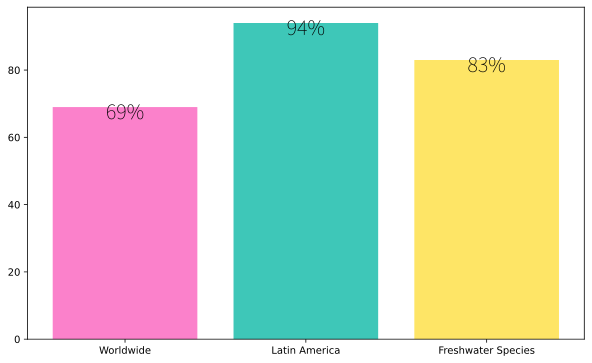
\includegraphics{sustainability_files/figure-pdf/cell-2-output-1.pdf}

Biodiversity loss is linked to overconsumption, weak legislation and
lack of oversight. (Crenna, Sinkko and Sala, 2019) recounts European
Union consumers' negative impact on biodiversity in countries where it
imports food. WWF (2022) case study highlights how 4 biodiverse regions
Cerrado in Brazil, Chaco in Argentina, Sumatra in Indonesia, and the
Cuvette Centrale in Democratic Republic of Congo are experiencing rapid
destruction due to consumer demand in the European Union. While the
European Union (EU) has recently become a leader in sustainability
legislation, biodiversity protection measures among private companies is
very low Marco-Fondevila and Álvarez-Etxeberría (2023).

Meanwhile, there is some progress in biodiversity conservation. UEBT
(2022) reports ``Biodiversity awareness is now at 72\% or higher in all
countries sampled, compared to only 29\% or higher across countries
sampled in 2009.''

Similarly to climate protection, the UN has taken a leadership role in
biodiversity protection. Unit (2023): The history of the United Nations
Convention on Biodiversity goes back to 1988, when the working group was
founded. UNEP (Tue, 12/20/2022 - 07:44): The Convention on Biodiversity
2022 (COP15) adopted the first global biodiversity framework to
accompany climate goals.

\paragraph{\texorpdfstring{\textbf{\emph{Biodiversity
Indicators}}}{Biodiversity Indicators}}\label{biodiversity-indicators}

Cutting edge research uses AI for listening to nature, assessing
biodiversity based on species' sounds in the forest. Millions of
detections of different species with machine learning passive acoustic
AI models, can also assess species response to climate change (AI for
Good, 2023; Guerrero et al., 2023).

May (2011) argues biodiversity loss is a concern for 3 points of views:

\begin{longtable}[]{@{}
  >{\raggedright\arraybackslash}p{(\columnwidth - 2\tabcolsep) * \real{0.2072}}
  >{\raggedright\arraybackslash}p{(\columnwidth - 2\tabcolsep) * \real{0.7928}}@{}}
\caption{From May (2011).}\tabularnewline
\toprule\noalign{}
\endfirsthead
\endhead
\bottomrule\noalign{}
\endlastfoot
View & \\
Narrowly Utilitarian & Biodiversity is a resource of genetic novelties
for the biotech industry. \\
Broadly Utilitarian & Humans depend upon biodiverse ecosystems. \\
Ethical & Humans have a responsibility to future generations to pass
down a rich natural world. \\
\end{longtable}

\paragraph{Forest and Deforestion}\label{forest-and-deforestion}

Around 27\% of Earth's land area is still covered by forests yet
deforestation is widespread all around the world; highest rates of
deforestation happened in the tropical rainforests of South America and
Africa, mainly caused by agricultural cropland expansion (50\% of all
deforestation) and grazing land for farm animals to produce meat
(38,5\%), totaling close to 90\% of global deforestation (Anon., 2022a).
Forests are a crucial part of Earth's carbon cycle and the main natural
CO\textsubscript{2} capture system; due to deforestation, Europe rapidly
losing its forest carbon sink (Frédéric Simon, 2022).

Afforestation is different from reforestation, which takes into account
biodiversity.

\begin{itemize}
\item
  Klosterman et al. (2022) using remote-sensing and machine-learning to
  assess reforestation potential; doesn't take into account political
  realities.
\item
  Global Forest Cover Change, Earth Engine Hansen et al. (2013)
\item
  1 billion tree project (Bastin et al., 2019; Anon., 2020; Greenfield
  and @pgreenfielduk, 2021)
\item
  Burning of biomass undermines carbon capture.
\end{itemize}

\paragraph{Air and Water Pollution is
Widespread}\label{air-and-water-pollution-is-widespread}

\begin{itemize}
\tightlist
\item
  Clean water and water pollution
\item
  Koch (2022) (\textbf{Need access! nyc times)}
\end{itemize}

Air pollution is widespread around the planet, with 99\% of Earth's
human population being affected by bad air quality that does not meet
WHO air quality guidelines, leading to health problems linked to 6.7
million premature deaths every year World Health Organization (2022).
Grounbreaking research by Lim et al. (2022) analyzed over 400000
individuals in England, South Korea and Taiwan establishes exposure to
2.5μm PM (PM2.5) air pollution as a cause for lung cancer. Bouscasse et
al. (2022) finds strong health and economic benefits across the board
from air pollution reduction in France. In Hannah Devlin (2022), prof
Tony Mok, of the Chinese University of Hong Kong: ``We have known about
the link between pollution and lung cancer for a long time, and we now
have a possible explanation for it. As consumption of fossil fuels goes
hand in hand with pollution and carbon emissions, we have a strong
mandate for tackling these issues -- for both environmental and health
reasons''.

Health and sustainability are inextricably linked. ``Human health is
central to all sustainability efforts.'', ``All of these (food, housing,
power, and health care), and the~stress~that the lack of them generate,
play a huge role in our health'' (Sarah Ludwig Rausch and Neha Pathak,
2021).

The main way to combat air pollution is through policy interventions.
MARIA LUÍS FERNANDES (2023) EU has legislation in progress to curb
industrial emissions. If legislation is in place, causing bad air
quality can become bad for business. Gu et al. (2023) links air
pollution to credit interest rates for business loans in China;
companies with low environmetal awareness and a history of environmental
penalties pay 12 percent higher interest rates.

Clean air is a requirement.

\paragraph{Climate Change Disasters}\label{climate-change-disasters}

\begin{itemize}
\item
  A comprehensive review of evidence from paleoclimate records until
  current time, including ocean, atmosphere, and land surface of points
  towards substantial climate change if high levels of greenhouse gas
  emissions continue, termed by the authors as \emph{climate
  sensitivity} (Sherwood et al., 2020).
\item
  (Anon., 2023b) The US Global Change Research Program comprehensive
  report to the US Congress links disaster-risk directly to global
  warming; for examples increased wildfires damage property, endager
  life and reduces air quality, which in effect increases health
  challenges.
\end{itemize}

Environmental activists have been calling attention to global warming
for decades, yet the world has been slow to act (McKibben, 1989).

\begin{itemize}
\item
  Flood risk mapping might lower property prices in at risk areas
  (Sherren, 2024).
\item
  In Taiwan disaster risk and hazard mapping, early warning systems, and
  comprehensive response save lives Tsai et al. (2021)
\end{itemize}

Global warming increases the risk of disasters and extreme weather
events. As extreme temperatures are increasingly commonplace, there's
increased risk of wildfires (Volkova, Roxburgh and Weston, 2021).
Summers of 2022 and 2023 were the hottest on record so far, with extreme
heat waves recorded in places around the world (Douglas, 2023; Falconer,
2023; National Oceanic and Atmospheric Administration (NOAA), U.S.
Department of Commerce, 2023; NOAA National Centers for Environmental
Information, 2023; Serrano-Notivoli et al., 2023; Venturelli et al.,
2023). As temperatures rise, certain cities may become uninhabitable for
humans (CBC Radio, 2021). The summer of 2023 saw extensive wildfires in
Spain, Canada, and elsewhere; rapidly moving fires destroyed the whole
city of Lāhainā in Hawaii {[}ADD CITATION{]}. The part of Earth where
the \emph{human climate niche} is becoming smaller (McKibben, 2023).
Some parts of South America have seen summer heat in the winter, with
heatwaves with temperatures as high as 38 degrees (Livingston, 2023).

\begin{itemize}
\tightlist
\item
  Observed changes in heatwaves (Perkins-Kirkpatrick and Green, 2023).
\item
  Word Economic Forums Global Risks Report 2024 paints a bleak picture
  of the future with expectations of increased turbulence across the
  board based on a survey of over 1400 topic experts World Economic
  Forum (n.d.)
\end{itemize}

Climate-related disasters can spur action as extreme weather becomes
visible to everyone. After large floods in South Korea in July 2023 with
many victims, president Joon promised to begin taking global warming
seriously and steer the country towards climate action Web (2023); AFP
(2023); Al Jazeera (2023). South Korea has a partnership with the
European Union European Commission (2023a).

The fossil energy production that's a large part of global CO2 emissions
has caused several high-profile pollution events. Large ones that got
international news coverage include Exxon Valdez and Deepwater Horizon.

\begin{itemize}
\tightlist
\item
  Chernobyl and Fukushima
\item
  the Great Pacific Garbage Patch
\item
  Lenton et al. (2023) quantifying human cost of global warming.
\item
  EJAtlas tracks environmental justice cases around the world Scheidel
  et al. (2020).
\item
  Disputes in Eerola (2022).
\end{itemize}

\paragraph{Carbon Accounting in Corporate
Industry}\label{carbon-accounting-in-corporate-industry}

\begin{itemize}
\item
  Watershed
\item
  The legislation has created an industry of CO\textsubscript{2}
  accounting with many companies like Greenly, Sustaxo, etc.
\item
  Quatrini (2021) sustainability assessments are complex and may give
  flawed results.
\item
  Nonetheles, CO\textsubscript{2} emission reduction has the added
  positive effect of boosting corporate morale (Cao, Li and Hasan,
  2023).
\end{itemize}

\subsubsection{Agroforestry \&
Permaculture}\label{agroforestry-permaculture}

\begin{itemize}
\tightlist
\item
  Agroecology Baltic Sea Action Group (2023)
\end{itemize}

Agroforestry plays an active role in achieving Sustainable Development
Goals (SDGs) (Ruba and Talucder, 2023);

\begin{itemize}
\item
  Food forests for regenerative food systems.
\item
  Irwin et al. (2023)
\item
  Yadav et al. (2023)
\item
  Low, G., Dalhaus and Meuwissen (2023)
\item
  Ollinaho and Kröger (2023) ``bioeconomy is not inherently sustainable
  and may pose considerable risks to biodiversity.''
\item
  De Queiroz-Stein and Siegel (2023)
\item
  Gamage et al. (2023) ``Organic food and drink sales in 2019 totaled
  more than 106 billion euros worldwide.''
\item
  ``Would you rather buy a DogeCoin or a regenerative food forest
  token?'' Curve Labs founder Pat Rawson quotes Shiller (2019) in ReFi
  podcast about Kolektivo. ReFi DAO (2022) (Use as a question for the
  survey?)
\end{itemize}

\subsubsection{Quality of Life}\label{quality-of-life}

\begin{itemize}
\item
  Kaklauskas et al. (2023)
\item
  Rieger et al. (2023) Integrated science of wellbeing
\item
  Fabris and Luburić (2022)
\item
  Sustainability is part of product quality. If a product is hurting the
  environment, it's a low quality product.
\end{itemize}

\subsubsection{Restoration Ecology}\label{restoration-ecology}

\begin{itemize}
\item
  Bioswales
\item
  Fischer et al. (2021) UN announced 2021--2030 the Decade on Ecosystem
  Restoration
\end{itemize}

\subsubsection{\texorpdfstring{\textbf{Environmental
DNA}}{Environmental DNA}}\label{environmental-dna}

\begin{itemize}
\item
  Ogram, Sayler and Barkay (1987) isolating cellular DNA from various
  sediment types.
\item
  Peter Andrey Smitharchive page (2024) describes
\end{itemize}

\subsubsection{Digital Twins}\label{digital-twins}

\begin{itemize}
\item
  We can use all the data being recorded to provide a Digital Twin of
  the planet, nature, ecosystems and human actions to help us change our
  behavior and optimize for planetary wellbeing.
\item
  The EU is developing a digital twin of Earth to help sustainability
  prediction and planning, integrating Earth's various systems such as
  climate, hydrology, ecology, etc, into a single model Anon. (2023c).
\item
  EU releases strategic foresight reports since 2020 European Commission
  (2023b)
\end{itemize}

\subsection{Mitigation \& Adaption}\label{mitigation-adaption}

Many companies are developing technologies for mitigation.

\paragraph{Cap \& Trade}\label{cap-trade}

The share of CO\textsubscript{2} emissions among people around the world
is highly unequal across the world (referred to as \textbf{\emph{Carbon
Inequality}}). (Chancel, 2022) reports ``one-tenth of the global
population is responsible for nearly half of all emissions, half of the
population emits less than 12\%''.

\begin{itemize}
\item
  One example is the ICT sector.
\item
  Bajarin (n.d.) Over 300 million PCs sold in 2022

  \begin{itemize}
  \tightlist
  \item
    Anon. (2021a) Estonian company ``sustainable lifecycle management of
    IT equipment''
  \item
    Ärileht (23.09.2022, 12:53) Recycle your phone, FoxWay and Circular
    economy for PCs.
  \item
    Zhou et al. (2022) ICT is an example of inequality, while emerging
    economies bear 82\% of the emissions, developed countries gain 58\%
    of value.
  \end{itemize}
\end{itemize}

\subsubsection{Emissions' Data}\label{emissions-data}

Data about green house gas emissions.

\begin{longtable}[]{@{}
  >{\raggedright\arraybackslash}p{(\columnwidth - 4\tabcolsep) * \real{0.4000}}
  >{\raggedright\arraybackslash}p{(\columnwidth - 4\tabcolsep) * \real{0.3167}}
  >{\raggedright\arraybackslash}p{(\columnwidth - 4\tabcolsep) * \real{0.2750}}@{}}
\caption{Comparing highest per capita CO\textsubscript{2} emissions
(mostly from oil producers) vs regional average per capita
CO\textsubscript{2} emissions vs total CO\textsubscript{2}
emissions(Crippa et al., 2020; Ivanova et al., 2020; World Resources
Institute, 2020; European Commission. Joint Research Centre., 2022; Liu,
Z. et al., 2023).}\tabularnewline
\toprule\noalign{}
\endfirsthead
\endhead
\bottomrule\noalign{}
\endlastfoot
Regional Avergage Per Capita Emissions (2020) & Highest Per Capita
Emissions (2021) & Highest Total Emissions (2021) \\
North America 13.4 CO\textsubscript{2}e tonnes & Palau & China \\
Europe 7.5 CO\textsubscript{2}e tonnes & Qatar & United States \\
Global Average 4.1 CO\textsubscript{2}e tonnes & Kuwait & European
Union \\
Africa and the Middle East 1.7 CO\textsubscript{2}e tonnes & Bahrain &
India \\
& Trinidad and Tobago & Russia \\
& New Caledonia & Japan \\
& United Arab Emirates & Iran \\
& Gibraltar & Germany \\
& Falkland Islands & South Korea \\
& Oman & Indonesia \\
& Saudi Arabia & Saudi Arabia \\
& Brunei Darussalam & Canada \\
& Canada & Brazil \\
& Australia & Turkey \\
& United States & South Africa \\
\end{longtable}

``The world's top 1\% of emitters produce over 1000 times more CO2 than
the bottom 1\%'' IEA (2023a)

Crippa et al. (2020) reports latest figures from the EU's Emissions
Database for Global Atmospheric Research (EDGAR)

The EU Copernicus satellite system reveals new greenhouse emissions
previously undetected (Daniel Värjö, 2022).

\subsubsection{Emissions Trading
Schemes}\label{emissions-trading-schemes}

From Carbon Offsets to Carbon Credits

Retiring CO\textsubscript{2} allowances

\begin{itemize}
\tightlist
\item
  Facilitating citizens' access to CO\textsubscript{2} emissions trading
  may be an efficient method to organize large-scale CO\textsubscript{2}
  retiring Rousse (2008)
\item
  ``A carbon credit represents one tonne of carbon dioxide that has been
  prevented from entering or has been removed from the atmosphere''
  (Anna Watson, 2023; \textbf{annawatsonDeepDiveCarbon2022?}).
\end{itemize}

As of 2023 there isn't a single global CO\textsubscript{2} trading
market but rather several local markets as described in the table below
Anon. (n.d.a).

\begin{longtable}[]{@{}
  >{\raggedright\arraybackslash}p{(\columnwidth - 4\tabcolsep) * \real{0.1149}}
  >{\raggedright\arraybackslash}p{(\columnwidth - 4\tabcolsep) * \real{0.0596}}
  >{\raggedright\arraybackslash}p{(\columnwidth - 4\tabcolsep) * \real{0.8213}}@{}}
\caption{CO\textsubscript{2} credit trading markets around the world
from Anon. (n.d.a).}\tabularnewline
\toprule\noalign{}
\endfirsthead
\endhead
\bottomrule\noalign{}
\endlastfoot
CO\textsubscript{2} Market & Launch Date & Comments \\
European Union & 2005 & EU: Araújo et al. (2020) \\
& & \\
South Korea & 2015 & \\
China & 2021 & China's national emissions trading scheme (ETS) started
in 2021 priced at 48 yuan per tonne of CO\textsubscript{2}, averaged at
58 yuan in 2022 (Liu, H., 2021; Ivy Yin, 2023). \\
United States of America & 2013 & No country-wide market; local
CO\textsubscript{2} markets in California, Connecticut, Delaware, Maine,
Maryland, Massachusetts, New Hampshire, New York, Rhode Island, and
Vermont \\
New Zealand & 2008 & New Zealand Rontard and Reyes Hernández (2022)
(need access, important ncku doesn't subscribe) \\
Canada & 2013 & \\
\end{longtable}

Most of the world is not part of a CO\textsubscript{2} market.

\begin{itemize}
\tightlist
\item
  (Sipthorpe et al., 2022) compares traditional and blockchain-based
  solutions to carbon trading.
\item
  (United Nations Environment Programme (UNEP), 2021) report. ``The
  Emissions Gap Report (EGR) 2021: The Heat Is On shows that new
  national climate pledges combined with other mitigation measures put
  the world on track for a global temperature rise of 2.7°C by the end
  of the century. That is well above the goals of the Paris climate
  agreement and would lead to catastrophic changes in the Earth's
  climate. To keep global warming below 1.5°C this century, the
  aspirational goal of the Paris Agreement, the world needs to halve
  annual greenhouse gas emissions in the next eight years.
\item
  (United Nations Environment Programme (UNEP), 2021) report ``If
  implemented effectively, net-zero emissions pledges could limit
  warming to 2.2°C, closer to the well-below 2°C goal of the Paris
  Agreement. However, many national climate plans delay action until
  after 2030. The reduction of methane emissions from the fossil fuel,
  waste and agriculture sectors could help close the emissions gap and
  reduce warming in the short term, the report finds. Carbon markets
  could also help slash emissions. But that would only happen if rules
  are clearly defined and target actual reductions in emissions, while
  being supported by arrangements to track progress and provide
  transparency.''
\item
  (United Nations Environment Programme, 2022) 2022 Emissions Gap
  report.
\end{itemize}

\subsubsection{Carbon Markets}\label{carbon-markets}

For the individual person, there's no direct access to
CO\textsubscript{2} markets, however there are different types of
brokers who buy large amounts of carbon credits and resell them in
smaller quantities to retail investors. ``Carbon pricing is not there to
punish people,'' says Lion Hirth Lion Hirth (n.d.). ``It's there to
remind us, when we take travel, heating, consumption decisions that the
true cost of fossil fuels comprises not only mining and processing, but
also the damage done by the CO\textsubscript{2} they release.''

\paragraph{\texorpdfstring{The Price of CO\textsubscript{2} Differs
Across
Markets}{The Price of CO2 Differs Across Markets}}\label{the-price-of-co2-differs-across-markets}

Stern (2022) reports carbon-neutral economy needs higher
CO\textsubscript{2} prices. Rennert et al. (2022): Carbon price should
be 3,6x higher that it is currently. Ritz (2022) argues optimal
CO\textsubscript{2} prices could be highly asymmetric, low in some
countries and high (above the social cost of CO\textsubscript{2}) in
countries where production is very polluting.

\begin{itemize}
\tightlist
\item
  iGenius (2020)
\item
  The total size of carbon markets reached 949 billion USD in 2023,
  including Chinese, European, and North American CO2e trading (LSEG and
  Susanna Twidale, 02/12/2024, 02:37 PM).
\end{itemize}

\paragraph{Compliance Markets}\label{compliance-markets}

\begin{longtable}[]{@{}ll@{}}
\caption{Compliance market CO\textsubscript{2} prices on August 12,
2023; data from (CarbonCredits, 2023; Ember, 2023; Trading Economics,
2023).}\tabularnewline
\toprule\noalign{}
\endfirsthead
\endhead
\bottomrule\noalign{}
\endlastfoot
Compliance Markets & Price (Tonne of CO\textsubscript{2}) \\
EU & 83 EUR \\
UK & 40 Pounds \\
US (California) & 29 USD \\
Australia & 32 USD \\
New Zealand & 50 USD \\
South Korea & 5.84 USD \\
China & 8.29 USD \\
& \\
\end{longtable}

\paragraph{Voluntary Carbon Markets}\label{voluntary-carbon-markets}

Voluntary Carbon Markets are \ldots{}

Voluntary Carbon Markets (VCM) lack standardization and transparency
(Ela Khodai, 2023).

\textbf{\emph{Carbon Credits}} are useful for private companies who wish
to claim \emph{carbon neutrality, climate positivity}, or other related
claim, which might be viewed in good light by their clients or allow the
companies to adhere to certain legislative requirements.

There are many companies which facilitate buy carbon credits as well as
a few organizations focused on carbon credit verification.

\begin{itemize}
\tightlist
\item
  In Estonia, startups Arbonic and Single.Earth are trialing this
  approach in several forests.
\item
  Carbon Credit Retirement?
\item
  Methodologies: Anon. (2022b)
\item
  KlimaDAO (2023) call for an open standard
\end{itemize}

\begin{longtable}[]{@{}ll@{}}
\caption{Voluntary market CO\textsubscript{2} prices on August 12, 2023;
data from (CarbonCredits, 2023).}\tabularnewline
\toprule\noalign{}
\endfirsthead
\endhead
\bottomrule\noalign{}
\endlastfoot
Voluntary Markets & Price (Tonne of CO\textsubscript{2}) \\
Aviation Industry Offset & \$0.93 \\
Nature Based Offset & \$1.80 \\
Tech Based Offset & \$0.77 \\
\end{longtable}

\paragraph{Fossil Fuels}\label{fossil-fuels}

Fossil fuels are what powers humanity as well as the largest source of
CO\textsubscript{2} emissions. IEA (2022) reports ``Global
CO\textsubscript{2} emissions from energy combustion and industrial
processes rebounded in 2021 to reach their highest ever annual level. A
6\% increase from 2020 pushed emissions to 36.3 gigatonnes''. As on June
2023, fossil fuel based energy makes up 82\% of energy and is still
growing Institute (2023). The 425 largest fossil fuel projects represent
a total of over 1 gigatons in CO\textsubscript{2} emissions, 40\% of
which were new projects Kühne et al. (2022). Tilsted et al. (2023)
expects the fossil fuel industry to continue grow even faster. In July
2023, the U.K. granted hundreds of new oil and gas of project licenses
in the North Sea (Anon., 2023d).

\paragraph{Renewable Energy}\label{renewable-energy}

\begin{itemize}
\tightlist
\item
  10 countries use almost 100\% renewable energy
\end{itemize}

There's ample evidence from several countries suggesting moving to
renewal energy brings environmental benefits:

\begin{itemize}
\item
  Amin et al. (2022) suggests ``removing fossil fuel subsidies and
  intra-sectoral electricity price distortions coupled with carbon taxes
  provides the highest benefits'' for both the economy and the
  environment in Bangladesh.
\item
  Luo et al. (2022) suggests using reinforcement learning to reduce
  energy use in cooling systems.
\item
  The true cost of products is hidden. The work is hidden.
\item
  Montreal protocol eradicates CfCs and the ozone holes became whole
  again.
\end{itemize}

\paragraph{Emission Scopes Organize Calculating
CO2e}\label{emission-scopes-organize-calculating-co2e}

The U.S. National Public Utilities Council (NPUC) decarbonization report
provides a useful categorization of \textbf{\emph{emission scopes}}
applicable to companies and for organizing emission reduction schemes
(National Public Utilities Council, 2022). For example, for consumers in
Australian states and territories in 2018, 83\% of the GHG emissions are
Scope 3, meaning indirect emissions in the value chain Goodwin et al.
(2023).

\begin{longtable}[]{@{}ll@{}}
\caption{From National Public Utilities Council (2022).}\tabularnewline
\toprule\noalign{}
\endfirsthead
\endhead
\bottomrule\noalign{}
\endlastfoot
Emission Scope & Emission Source \\
Scope 1 & Direct emissions \\
Scope 2 & Indirect electricity emissions \\
Scope 3 & Value chain emissions \\
\end{longtable}

One's scope 3 emissions are someone else's scope 1 emissions.

\begin{itemize}
\tightlist
\item
  Mapping pollution sources in China Xie et al. (2021)
\end{itemize}

\paragraph{Carbon Capture}\label{carbon-capture}

Many technology startups focused on climate solutions (often referred to
as climatech by the media), have proposed a range of approaches to
CO\textsubscript{2} reduction in the atmosphere.

\begin{itemize}
\item
  Vitillo et al. (2022) illustrates how direct air capture of
  CO\textsubscript{2} is difficult because of low concentration and
  CO\textsubscript{2} capture at the source of the emissions is more
  feasible.
\item
  Gaure and Golombek (2022) simulate a CO\textsubscript{2} free
  electricity generation system in the European Union where ``98\% of
  total electricity production is generated by wind power and solar; the
  remainder is covered by a backup technology.''. The authors stipulate
  it's possible to power the EU without producing CO\textsubscript{2}
  emissions.
\item
  \textbf{Important: ``creating sustainability trust in companies in
  realtime''}
\item
  Howard et al. (2017) argues Oceans play crucial role in carbon
  capture.
\end{itemize}

\paragraph{\texorpdfstring{Social Cost of Carbon Measures Compound
CO\textsubscript{2}
Impact}{Social Cost of Carbon Measures Compound CO2 Impact}}\label{social-cost-of-carbon-measures-compound-co2-impact}

Sustainability is filled with complexities, where CO\textsubscript{2}
emission is compounded by biodiversity loss, child labor, slavery,
poverty, prostitution, dangerous chemicals, and many other issues become
intertwined (TEDx Talks, 2020). One attempt to measure these
complexities, is the Social Cost of Carbon (SCC) which is defined as
``additional damage caused by an extra unit of emissions'' (Zhen, Tian
and Ye, 2018; Kornek et al., 2021). For example the cost of damages
caused by ``one extra ton of carbon dioxide emissions'' (Stanford
University, 2021). SCC variations exists between countries (Tol, 2019)
and regions (Wang, Y., Ma and Wang, 2022).

\begin{itemize}
\item
  As shown in the Phillipines by (Cheng and Han, 2022), with increasing
  extreme weather events, ``businesses are more likely to emerge in
  areas where infrastructure is resilient to climate hazards''.
  (Jerrett, Jina and Marlier, 2022) says, In California, ``Wildfires are
  the second most important source of emissions in 2020'' and
  ``Wildfires in 2020 negate reductions in greenhouse gas emissions from
  other sectors.''
\item
  (Lin et al., 2022) says, apart from CO\textsubscript{2}, reduction of
  other atmospheric pollutants, such as non-CO\textsubscript{2}
  greenhouse gases (GHGs) and short-lived climate pollutants (SLCPs) is
  required for climate stability.
\item
  (Wang, T.-P. and Teng, 2022): Quantifying climate damage proposes
  scenarios of climate damage.
\end{itemize}

\paragraph{Country-Level Nationally Determined Contributions
(NDCs)}\label{country-level-nationally-determined-contributions-ndcs}

\begin{itemize}
\tightlist
\item
  UNFCCC. Secretariat (2022) The State of Nationally Determined
  Contributions
\end{itemize}

While most countries have not reached their Nationally Determined
Contributions, the Climate Action Tracker data portal allows to compare
countries (Climate Analytics and NewClimate Institute, 2023).

\begin{longtable}[]{@{}ll@{}}
\caption{Climate Action Tracker's country comparison of the 10 top
polluters' climate action.}\tabularnewline
\toprule\noalign{}
\endfirsthead
\endhead
\bottomrule\noalign{}
\endlastfoot
Country or Region & NDC target \\
China & Highly insufficient \\
Indonesia & Highly insufficient \\
Russia & Critically insufficient \\
EU & Insufficient \\
USA & Insufficient \\
United Arab Emirates & Highly insufficient \\
Japan & Insufficient \\
South Korea & Highly insufficient \\
Iran & Critically insufficient \\
Saudi Arabia & Highly insufficient \\
\end{longtable}

\begin{itemize}
\tightlist
\item
  Fransen et al. (2022) notes that the majority of Nationally Determined
  Contributions (NDCs) are dependent on financial assistance from the
  international community.
\end{itemize}

TODO

\begin{itemize}
\tightlist
\item
  ``triple turn''
\item
  lack of transparency
\item
  Call for GOP contributors' transparency
\end{itemize}

\paragraph{SDGs}\label{sdgs}

\begin{itemize}
\item
  SDGs need to discussed in their totality Popkova et al. (2022).
\item
  German Institute of Development and Sustainability (IDOS) connects
  SDGs to NDCs. Dzebo, Iacobuţă and Beaussart (2023)
\item
  International Energy Agency (IEAs), Decarbonisation Enablers IEA
  (2023b)
\end{itemize}

\subsection{Eco-Design}\label{eco-design}

\textbf{\emph{Designing for Sustainability aka Circular Design or
Eco-Design}} encompasses all human activities, making this pursuit an
over-arching challenge across all industries also known as circular
economy. Assuming that as individuals we want to act in a sustainable
way, how exactly would be go about doing that?

\begin{itemize}
\item
  ``Evolution of design for sustainability: From product design to
  design for system innovations and transitions''
\item
  de Otazu et al. (2022) \textbf{Life Cycle Assessment and environmental
  impact analysis are needed to provide eco-design scenarios.}
\item
  European Parliament (2022) proposal ``On 30 March 2022, the European
  Commission put forward a proposal for a regulation establishing a
  general framework for setting eco-design requirements for sustainable
  products, repealing rules currently in force which concentrate on
  energy-related products only.'' Virginijus Sinkevičius, EU
  Commissioner for the Environment, Oceans and Fisheries, is quoted as
  describing eco-design ``respects the boundaries of our planet''
  European Commission (2022a)
\item
  Forming an emotional bond with the product makes it feel more valuable
  (Zonneveld and Biggemann, 2014). This has implications for
  sustainability as the object is less likely to be thrown away.
\end{itemize}

\subsubsection{Regenerative design}\label{regenerative-design}

\begin{itemize}
\tightlist
\item
  Dematerialize economies is not enough.
\end{itemize}

\subsubsection{Biomimicry}\label{biomimicry}

\begin{itemize}
\tightlist
\item
  following nature
\end{itemize}

\subsubsection{Biodesign}\label{biodesign}

MIT is a source of many fantastic innovations.

\begin{itemize}
\item
  Neri Oxman, biomaterials MIT media lab, 15. sept. 2020
\item
  Neri Oxman's expressions: ``ecology-indifferent'', ``naturing'',
  ``mother naturing'', ``design is a practice of letting go of all that
  is unnecessary'', ``nature should be our single client''.
\item
  Use imagination
\item
  Societal movements change things: implication for design: build a
  community
\item
  Processes sustain things: implication for design: built an app
\end{itemize}

\subsubsection{AI-Assisted Design Enables Desiging for
Sustainability}\label{ai-assisted-design-enables-desiging-for-sustainability}

Gupta et al. (2023) argues software is key to building more sustainable
products, already for decades. More recently, companies like AutoDesk
are putting CO\textsubscript{2} calculations inside their design
software.

\begin{itemize}
\tightlist
\item
  AI has the potential to provide the parameters for sustainability.
  Singh and Sarkar (2023) proposes an AI tool for deciding the suitable
  life cycle design parameters.
\item
  Anon. (n.d.b): ``Sustainability starts in the design process, and AI
  can help''.
\end{itemize}

\subsubsection{Circular Economy}\label{circular-economy}

Circular economy is a tiny part of the world economy. Circle Economy
(2022) reports only 8.6\% of world economy is circular and \emph{100B
tonnes of virgin materials} are sourced every year.

\begin{itemize}
\item
  McDonough and Braungart (2002) book
\item
  McGinty (Thu, 08/06/2020 - 11:25): How to Build a Circular Economy
\item
  Dull (2021) book
\item
  Chapman (2009) argues in his seminal paper (and later in his book) for
  \textbf{\emph{``Emotionally Durable Design''}}, the simple idea that
  we hold to things we value and thus they are sustainable. We don't
  throw away a necklace gifted to us by mom, indeed this object might be
  passed down for centuries. Rose (2015) has a similar idea, where
  \textbf{\emph{``Enchanted Objects''}} become so interlinked with us,
  we're unlikely to throw them away.
\item
  Growing public understanding of how nature works and intersects with
  our use of money.
\item
  Hedberg and Šipka (2021) argues digitization and data sharing is a
  requirement for building a circular economy.
\item
  ``Circular Petrochemicals'' Lange (2021)
\item
  Supply chain transparency enables stakeholder accountability (Fox,
  2007; Doorey, 2011; Circularise, 2018).
\item
  Recycling Critical Raw Materials, digitalisation of mining allows
  enhance the reliability of supply chains (CRM Alliance, 2020).
\item
  EIT RawMaterials
\end{itemize}

\subsection{Policy Context}\label{policy-context}

\begin{itemize}
\item
  ``In the context of the EU Plastics Strategy, the European Commission
  has launched a pledge to increase the use of recycled content to 10
  million tons by 2025. To address this, Circularise Plastics Group
  launched an ``Open Standard for Sustainability and Transparency''
  based on blockchain technology \& Zero-knowledge Proofs'' Circularise
  (2020a)
\item
  ``data-exchange protocol with privacy at its heart'' Circularise
  (2020b)
\item
  EU AI Law Lomas (2024)
\end{itemize}

\subsubsection{The Policy Context in Europe From 2023 to
2030}\label{the-policy-context-in-europe-from-2023-to-2030}

\begin{figure}[H]

{\centering \includegraphics[width=0.8\textwidth,height=\textheight]{./images/eu-policy-context.png}

}

\caption{EU Policy Context Timeline}

\end{figure}%

We have an opportunity to re-imagine how every product can be an
eco-product and how they circulate in our circular economy.

Timeline of the Policy Context:

\begin{itemize}
\item
  In 2019 by the von der Leyen commission adopted the European Union
  (EU) \textbf{Green Deal} strategy.
\item
  In 2021 the Commision proposed a goal of reducing CO2e emissions by
  55\% by 2030 under the \emph{Fit for 55} policy package consisting of
  a wide range of economic measures.
\item
  In November 2022, the proposal was adopted by the EU Council and EU
  Parliament with an updated goal of 57\% of CO2e reductions compared to
  1990. This proposal is set to become a binding law for all EU member
  countries (European Commission (2019a); European Commission (2019b);
  Anon. (2022c); European Council (2022)).
\item
  In March 2022, the EU Circular Economy Action Plan was adopted,
  looking to make sustainable products \emph{the norm} in EU and
  \emph{empowering consumers} as described in European Commission
  (2022b). Each product covered by the policy is required to have a
  \textbf{\emph{Digital Product Passport}} which enables improved
  processing within the supply chain and includes detailed information
  to empower consumers to understand the environmental footprint of
  their purchases. It's safe to say the large majority of products
  available today do not meet these criteria.
\end{itemize}

\paragraph{Wellbeing Economy Governments is an Example of Country-level
Collaboration}\label{wellbeing-economy-governments-is-an-example-of-country-level-collaboration}

\begin{itemize}
\tightlist
\item
  Finland, Iceland, New Zealand, Scotland, Wales, Canada
  https://weall.org/wego
\end{itemize}

\subsubsection{European Green Deal}\label{european-green-deal}

\begin{itemize}
\tightlist
\item
  Anon. (2021b)
\item
  Switch2Green (2023)
\end{itemize}

It's up to legislators to provide sustainable products on our
marketplace\ldots{} but until we do, use the green filter.

\begin{itemize}
\tightlist
\item
  One of the EU goals is reducing consumption
\item
  Tacking our consumption habits
\item
  Europe is the hotbed of sustainability
\item
  Iman Ghosh (2020)
\item
  Lamoureux (2018) Florida sustainable companies
\item
  MICHAEL HOULIHAN and BONNIE HARVEY (2018) customers prefer sustainable
  companies
\item
  Rajagopalan and Landrigan (2023): In the US, the \emph{Inflation
  Reduction Act} provides funding to development of decarbonizing
  technologies and includes plans to combat air pollution, reduce green
  house gases and address environmental injustices.
\end{itemize}

\subsubsection{Eco-Design is a Key EU Sustainable Policy Design
Tool}\label{eco-design-is-a-key-eu-sustainable-policy-design-tool}

A large part of the proposal by Commission et al. (2014) is
\textbf{\emph{eco-design}}, as a large part of product lifecycle
environmental impact is defined in the design process.

\begin{longtable}[]{@{}lll@{}}
\caption{Eco-design framework proposes 9 values to strive for in high
quality products.}\tabularnewline
\toprule\noalign{}
\endfirsthead
\endhead
\bottomrule\noalign{}
\endlastfoot
Quality & & \\
Durable & Reparable & Easy to recycle \\
Reusable & Easy to maintain & Energy efficient \\
Upgradable & Easy to refurbish & Resource efficient \\
\end{longtable}

\subsubsection{Sustainbility Policy is Shifting Around the
World}\label{sustainbility-policy-is-shifting-around-the-world}

Politics matters in sustainability.

In the European Union (EU), a wide range of legislative proposals,
targets, organizations, and goals already exists across diverse
countries. Upcoming laws aim to harmonize approaches to sustainability
and raise standards for all members states, in turn influencing
producers who wish to sell in the EU common market.

\begin{itemize}
\item
  In Brazil, deforestation fell 60\% in 1 year, based on remote
  satellite reconnaissance, after the election of a more pro-environment
  leadership Watts (2023).
\item
  Anon. (n.d.c) report: The EU has a \textbf{\emph{taxonomy of
  environmentally sustainable economic activities}} published by the
  Technical Expert Group (TEG) on sustainable finance.
\item
  The proposal for a Nature Restoration Law by the European Commission
  requiring member countries to restore 20\% of EU's degraded ecosystems
  by 2030 and full restoration by 2050 has not yet passed Anon. (2023e)
  and is facing a backlash David Pinto (2023).
\item
  Manzardo et al. (2021) \textbf{(need access!)}
\item
  Iñarra et al. (2022) \textbf{(need access!)}
\item
  Munaro, Tavares and Bragança (2022) \textbf{(need access!)}
\item
  Bassani et al. (2022) \textbf{(need access!)}
\item
  Van Doorsselaer (2022) \textbf{(need access!)}
\item
  Nuez, Ruiz-García and Osorio (2022) shows how electric vehicles may
  increase CO\textsubscript{2} emissions in some areas, such as Canary
  Islands, where electricity production is polluting.
\item
  Rossi, Cappelletti and Germani (2022) shows how introducing
  sustainability early in the design process and providing scenarios
  where sustainability is a metric, it's possible to achieve more
  eco-friendly designs.
\item
  Tiernan et al. (2022) microplastics are a real concern
\item
  Arranz, Sena and Kwong (2022) developing circular economy is really
  complex
\item
  Cheba et al. (2022)
\item
  Ruiz-Pastor et al. (2022)
\item
  Miyoshi et al. (2022) takes the example of ink toner bottles and shows
  in a case study how standardized compatibility between older and newer
  systems can save resources and results in sustainability savings.
\item
  Finding green products and supporting companies making them
\item
  Supporting legislative changes
\item
  Track you consumption, saving, investing. Shift balance towards saving
  and investing.
\item
  Nastaraan Vadoodi (2022)
\item
  European Commission (2022c) Ecodesign for sustainable products
\end{itemize}

\subsubsection{Waste Generation is Still
Increasing}\label{waste-generation-is-still-increasing}

Liu, K. et al. (2023) reports, e--waste is growing 3\%--5\% every year,
globally. (Thukral and Singh, 2023) identifies several barriers to
e-waste management among producers including lack of awareness and
infrastructure, attitudinal barriers, existing \emph{informal} e-waste
sector, and the need for an e-waste license.

\subsubsection{Extended Producer Responsibility Enables Compannies to be
Resposible}\label{extended-producer-responsibility-enables-compannies-to-be-resposible}

Extended Producer Responsibility (EPR) is a policy tool first proposed
by Thomas Lindhqvist in Sweden in 1990 {[}ADD CITATION{]}, aimed to
encourage producers take responsibility for the entire life-cycle of
their products, thus leading to more eco-friendly products. Nonetheless,
EPR schemes do not guarantee circularity and may instead be designed
around fees to finance waste management in linear economy models
(Christiansen, Hasse and Tønder, 2021). The French EPR scheme was
upgraded in 2020 to become more circular (Jacques Vernier, 2021).

In any case, strong consumer legislation (such as EPR) has a direct
influence on producers' actions. For example, in HKTDC Research (2022),
the Hong Kong Trade Development Council notified textile producers in
July 2022 reminding factories to produce to French standards in order to
be able enter the EU market. Peng, Shi and Tong (2023) finds that the
\textbf{\emph{Carbon Disclosure Project}} has been a crucial tool to
empower ERP in Chinese auto-producers.

\begin{itemize}
\tightlist
\item
  The success of EPR can vary per type of product. For car tires, the
  EPR scheme in the Netherlands claims a 100\% recovery rate
  Campbell-Johnston et al. (2020).
\end{itemize}

One type of legislation that works?

\begin{itemize}
\item
  Steenmans and Ulfbeck (2023) Argues for the need to engage companies
  through legislation and shift from waste-centered laws to product
  design regulations.
\item
  In Europe, there's large variance between member states when in comes
  to textile recycling: while Estonia and France are the only EU
  countries where separate collection of textiles is required by law, in
  Estonia 100\% of the textiles were burned in an incinerator in 2018
  while in France textiles are covered by an Extended Producer
  Responsibility (EPR) scheme leading to higher recovery rates (Ibid).
\item
  Greyparrot AI to increase recycling rates Natasha Lomas (2024)
\end{itemize}

\subsubsection{Return, Repair, Reuse}\label{return-repair-reuse}

\begin{itemize}
\tightlist
\item
  There's a growing number of companies providing re-use of existing
  items.
\item
  Anon. (n.d.d) For example, Swap furniture in Estonia
\end{itemize}

Bring back your bottle and cup after use.

\begin{itemize}
\tightlist
\item
  Ruiz-Pastor and Mesa (2023) proposes a \textbf{product repairability
  index (PRI)}
\item
  Formentini and Ramanujan (2023)
\item
  Recycling (Lenovo, 08-29-22) ``rethinking product design and inspiring
  consumers to expect more from their devices''
\item
  ``design is a tool to make complexity comprehensible'' like the
  Helsinki chapel. there's either or a priest or a social worker. it's
  the perfect public service. ``limit the barrier of entry for people to
  discover''. elegant.
\item
  Zeynep Falay von Flittner (n.d.)
\end{itemize}

\subsubsection{Packaging}\label{packaging}

Packaging is a rapidly growing industry which generates large amounts of
waste Ada et al. (2023). Bradley and Corsini (2023): ``Over 161 million
tonnes of plastic packaging is produced annually.''

\begin{itemize}
\tightlist
\item
  Anon. (2022d)
\item
  Anon. (2022e)
\item
  Anon. (2010)
\item
  (Lerner, 2019) Coca Cola plastic pollution. ESG ratings have faced
  criticism for lack of standards and failing to account for the
  comprehensive impact a company is having. (Foley et al., 2024) notes
  how Coca Cola fails to account the supply chain water usage when
  reporting becoming ``water neutral'' and calls on companies to release
  more detailed information.
\item
  Anon. (n.d.e)
\end{itemize}

\subsubsection{Factories Can Become More
Transparent}\label{factories-can-become-more-transparent}

\begin{itemize}
\item
  Regional supply chains for decarbonising steel: ``co-locating
  manufacturing processes with renewable energy resources offers the
  highest energy efficiency and cost reduction'' Japanese-Australia
  study s Devlin and Yang (2022)
\item
  Transparency about the polluting factories where the products come
  from.. the product journey
\item
  virtual factories
\item
  Tracing emissions from factory pipes\ldots{} what's the app?
\item
  Factories should be local and make products that can be repaired.
\item
  Carbon-neutral factories ``made in carbon-neutral factory'' list of
  products
\item
  Stefan Klebert (2022)
\item
  VDI Zentrum Ressourceneffizienz (2020)
\item
  Anon. (n.d.f) and Anon. (n.d.g) CO\textsubscript{2} neutral factories?
\item
  (Anon., n.d.h; Anon., n.d.i) CO\textsubscript{2} neutral websites
\item
  Eric fogg (2020) Lights-Out Manufacturing
\item
  Mowbray (2018) ``World's first free digital map of apparel factories''
\item
  Anon. (n.d.j) Factory compliance - Fair Factories
\item
  Planet Factory
\item
  Anon. (n.d.k) Plastic waste makers index, sources of plastic waste
\end{itemize}

\subsection{Design Implications}\label{design-implications}

\begin{longtable}[]{@{}
  >{\raggedright\arraybackslash}p{(\columnwidth - 2\tabcolsep) * \real{0.0625}}
  >{\raggedright\arraybackslash}p{(\columnwidth - 2\tabcolsep) * \real{0.9375}}@{}}
\caption{Implications}\tabularnewline
\toprule\noalign{}
\endfirsthead
\endhead
\bottomrule\noalign{}
\endlastfoot
Category & Implication \\
Transparency

Speed & In unison, the reviewed technologies and practices move us
closer to enabling \emph{realtime ESG}: up-do-date transparent
information about how our product are produced. Realtime ESG is a
building block to enable consumers and investors make more accurate,
real-world purchase decisions. \\
Pollution

Actionability & \emph{People live in the polluted areas are so used to
it. What app to wake them up? ``You live in a highly polluted area.
Here's the TOP 10 companies causing pollution. Here's what you can
do.''} \\
Health Tracking & Blood testing and biomarkers allow people to track
their health. I'm introducing the concept of `eco-markers' to follow the
sustainability of human activities. \\
Circular Economy & AI can help us make sense of the vast amounts of
sustainability data generated daily. \\
EPR & ERP and CDP data should be part of Green Filter. \\
& \\
& \\
& \\
& \\
& \\
\end{longtable}




\end{document}
